% This is the main report file

\documentclass{acm_proc_article-sp}
\usepackage[utf8]{inputenc}
\usepackage{listings}
\begin{document}

\title{02333 Parallel and Real-time Systems F10}
\subtitle{[Report on the work done in this course]
\titlenote{This report should also be available online at \texttt{www.retrospekt.dk/02333report}}}

\numberofauthors{4} %  in this sample file, there are a *total*
\author{
% 1st. author
\alignauthor
Andreas Rask Jensen\\
%       \affaddr{}\\
%       \affaddr{}\\
       \email{s083165@student.dtu.dk}
% 2nd. author
\alignauthor
Demmus Hentze Højgaard\\
       \email{s062591@student.dtu.dk}
% 3rd. author
\alignauthor
Hjallgrim Gunnar Mohr Hentze\\
       \email{s062418@student.dtu.dk}
\and  % use '\and' if you need 'another row' of author names
% 4th. author
\alignauthor 
Kim Rostgaard Christensen\\
       \email{s084283@student.dtu.dk}
}

\maketitle

\begin{abstract}
%Abstract; A brief summary of all of the report including the conclusion section
%but excluding the acknowledgements, references and any appendixes.
The purpose of this report is to describe in detail how we implemented the tasks in the course. The overall goal is to build a tiny operating system using the technologies also available in contemporary, widely used operating systems. We have decided to name the operating system GunKiAnDem. Our mascot is a walking stick (figure~\ref{fig:mascot}) Because we are using a skeleton code, and it kind of looks like a skeleton. 
\begin{figure}
\centering

\epsfig{file=fig/mascot.eps, height=0.5in}
\caption{The GunKiAnDem mascot}
\label{fig:mascot}
\end{figure}
\end{abstract}
% XXX Should this be here? 
% A category with the (minimum) three required fields
%\category{H.4}{Information Systems Applications}{Miscellaneous}
%A category including the fourth, optional field follows...
%\category{D.2.8}{Software Engineering}{Metrics}[complexity measures, performance measures]

%\terms{Report}

%\keywords{ACM proceedings, \LaTeX, text tagging} % NOT required for Proceedings


\section{Introduction}

%Introduction; A discussion putting the work into context and discussing the
%background of the work. The section should include any problem statements
%addressed, a very brief summary of the work carried out, the most import ant
%results and the most important conclusions. The section should end with a
%description of the report structure.


%\section{Related work}
%%Related work; A discussion of any material not background but still related to
%the report.


%Body; A number of sections describing the work done.

\section{System calls}
Task B1 is to implement a system call. This is a pretty fundamental feature in operating systems.\\

When designing an operating system you will soon run into thoughts about security. How would you secure that only system related activities
can access the system's resources directly? Easy, some might say. Just divide it into two areas with different privilege level. 
In operating systems those two levels are called user- and kernel mode. Not all operating systems have this split, but if you have a
 lot of 3rd party development you ought to make this split.\\
Programs running in kernel mode have direct access to all I/O devices, memory and so forth. This gives a lot of possibilities (-to mess something up).\\
Programs running in user mode do not have the same privileges and need therefore to have some kind of service specified in order to communicate with I/O and get extra memory. This ``API'' is called system calls. System calls are a set of commands that the operating system listens for and when these are called the system supplies the caller with the service applied for.\\
When a syscall is invoked, the CPU registers is pushed on the stack and the OS switches to kernel mode. The kernel uses a macro that calls some low-level assembler code in order to achieve this.


\begin{figure}
\centering
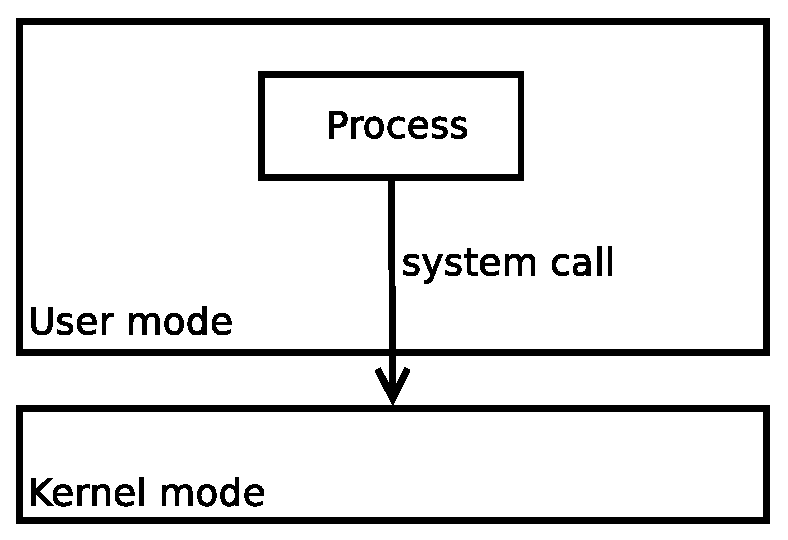
\epsfig{file=fig/Kernel_Mode.eps, height=1in}
\caption{Invoking a system call}
\label{fig:kernel_mode}
\end{figure}

\subsection{Reflections}

\subsubsection*{What kind of operating system is it?}
Tanenbaum and Woodhull describes three major types of operating system kernel types; monolithic, mico and exo.\\
The microkernel is based on the design philosophy that everything is implemented as a service, meaning that things like process management is done
in userspace and these services communicate via an IPC scheme (see section \ref{sec:ipc}).\\
%The exokernel is type of kernel that serves as a kernel on top other kernels in a hypervisor way\\
The monolithic kernel is proportionally weak in design pattern as microkernels is strong. They pretty much go by the ``anything goes'' design 
strategy. Our system is a monolithic operating system. Nothing is implemented as a service as in a microkernel or takes on any of the
characteristics of an exokernel.

%Draw a figure of the organization of the system. Relate the organization of the system to the different types of operation systems discussed in the text book by Tanenbaum and Woodhull. What kind of operating system is it?  Why?

\subsubsection*{Which portion execute in kernel mode? Which portions in user mode? What is the difference between user and kernel mode?}
All system calls is run in kernel mode. The kernel mode has access to system resources user mode doesn't

\subsubsection*{How is the kernel invoked from the user-level program? Explain and elaborate!}
The kernel is invoked through system calls. When a syscall is invoked, the CPU registers is pushed on the stack and switches to kernel mode. The kernel uses a macro that calls some low-level assembler code.

\subsubsection*{How is control passed back to the user-level program? Explain and elaborate!}

When the syscall returns, the stack is pushed back into the registers and the computer returns to user mode and continues the execution of the
program that did the system call.

\subsection{Test}
The executing program is to make the system call\\ “SYSCALL\_VERSION” where the kernel version should be printed to the bochs console. This desired result was achieved as defined in task definition, and the test was a success.
\label{sec:system_calls}

\section{Processes}
Task B2 was to implement process handling in out operating system. Lets look a bit closer on the concept of processes before discussing the implementation.
\subsubsection{The process concept}
A process is a in an instance of a program (an executable) that runs in an operating system environment, 
and returns to this operating system upon completion. Hence, the operating system is the one resposible for 
creating new processes and terminating them. An analogy to this is the a java object, being an instance of a java class.\\
The process is therefore nothing more than a container for resources reserved to the process by the operating system. \\

\subsubsection{The thread concept}
A thread is the part of the process container responsible for executing the program.

So, the operating system need to keep track of the running processes and take care of creating and terminating the processes. 
For this, we have added two system calls; create and terminate.

\begin{figure}
\centering
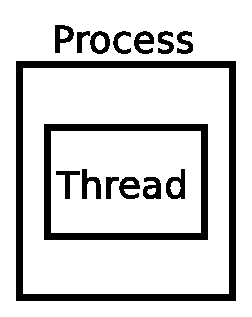
\epsfig{file=fig/Thread_Model_single.eps, width=0.5in}
\caption{Our thread model}
\end{figure}

\subsubsection*{The create system call}
To implement this, we need to keep track of the running processes. This is handled by a process table that contains structures holding information about an individual process. \\
Processes are executed invoking this system call by executing a piece of assembler code that calls a named procedure called ``main'' and then calls terminate when main is done executing.
\subsubsection*{The terminate system call}


\subsubsection{Reflections}

\subsubsection*{How is the system booted?}
Our virtual pc starts a BIOS that searches for a bootloader (in our case Grub), that then loads the kernel image to memory from a harddisk - or in our case a disk image. The kernel image 
\subsubsection*{How are processes created from executable files?}
The kernel finds all executable files and loads them to memory, storing a pointer to the first instruction for each process.

\subsubsection*{How does a daemon (process) differ from processes studied in this task?}
Our processes runs ``interactively'' and daemons runs in the background. Otherwise they share the fact that they are started at bootup by the os.

\label{sec:processes}

\section{Scheduling}
%concepts
Task B3 was to implement a non-premptive scheduler. We will first look into at what a scheduler is and what it does.

\subsubsection{The scheduler}
A conservative definition of a CPU says that it executes code in a linear form, meaning that all program code needs to be written/executed sequentially. Therefore there can only be executed one program at once, using up all of the CPU's processing power, which often is in abundance. Today most computers have the ability to run many programs simultaneously without significant loss of performance or user experience.\\
\\
This is made possible by the scheduler, whose job is to divide the processing power of the CPU to the many processes and threads that may require it. The "simple" CPU still only manages to run its assigned code sequentially, but the scheduler can assign what code to run - That's its job.
\\
\\
\\
% Agreed - but we should write this in a comment
% !!!!!!Maybe write a short intro to scheduling algorithms!!!!!!!!
\subsubsection{Non-preemptive}
Threads are allowed to run until it is finished or goes into blocked state on its own. A thread may for example block when requesting an I/O operation or calling the sleep system call.
\\
This means that any other thread will have to wait indefinitely until all preceding threads have gone into blocked state or have finished. 

\subsubsection{Preemptive}
Instead of allowing threads to run indefinitely, we halt them during execution to allow another thread to run. For this to be viable, a hardware interrupt is required. When the scheduler interrupt is received by the CPU, it is handled by the scheduler interrupt code. The scheduler then saves all the relevant registers, including the program counter. This is referred to as a context switch, and allows return the thread and its state, at any time.

\subsubsection{Round robin}
Now that the scheduling concept is defined, we need to figure out which thread to run and when. There are many scheduling algorithms defined, all with different strengths and weaknesses. Our implementation is referred to as round robin and is a very simple in that is only cycles thru all threads in the ready state and assigns them CPU runtime. The round robin algorithm has no prioritizing in its basic implementation, and therefore all threads are treated equally in the queue and no thread is skipped or delayed CPU time.

\subsubsection{Priority}
For some "critical" applications it is more important that it gets more CPU time. These critical applications often need this extra attention, so that the user experience isn't negatively affected. An example of this is the mouse cursor, which needs to move seamlessly across the screen in a single flowing motion. Therefore many algorithms support thread prioritizing in some form, allowing highest priority threads ahead of all others with lower priority.

\subsubsection{Process states}
In this section we will explain a little about the different states that processes can have when being handled by the scheduler. Since our implementation of the kernel is able to handle multiple threads per process, we will be referring to thread states, as appose to single-threaded-processes. This just means that we do not look at processes, but just the states of individual threads. We will also in this section make the assumption, that a scheduler implements some kind of time-sharing for the CPU, so that each thread gets the same amount of processing time
\\
\\
When running multiple threads with the help of a scheduler, the CPU processing time is reduced, each time a thread is added to the scheduler queue. Since CPU time is precious, it is good practice to not waste resources on threads that don't require processing. Probably the simplest example is when code that needs to sleep/pause/wait before continuing its code execution. The program can in this case voluntary make a call to the operating system telling it to skip all its execution for a designated time period. This is also referred to as setting the thread state to blocked.
\\
\\
Another reason for halting execution is when some kind of data is missing, which is vital for continue execution. This could be that an application is waiting for I/O data, and a time delay is on that operation. Instead of having the application check for incoming data at timed intervals, we could have the operating system handle the I/O call, and block the thread until the data is available.
\\
\\
Threads can be in one of three states; running state, ready state or blocked state.
When a thread is in the running state, it is being executed by the CPU. It can from this state go to block or ready, depending on the circumstances. The ready state is for threads that are waiting for CPU time. It is then up to the scheduler which threads with ready state are executed by putting them in running state. Threads that already are in the blocked state and are designated to be run are returned to the ready state, and the scheduler takes over, as with all other threads in ready state.
\\
\\
\begin{figure}
\centering
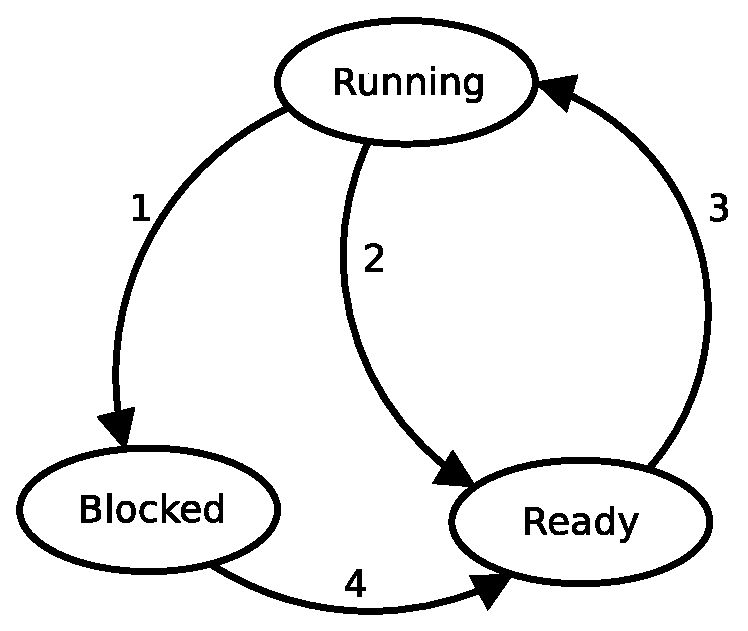
\epsfig{file=fig/Process_states.eps, height=1.5in}
\caption{Process states}
\label{fig:process_states}
\end{figure}

\subsubsection{Implementation}
\subsubsection*{scheduler.c}
The non-preemptive scheduler is implemented in the scheduler.c file, which is then included in the kernel.c file, in the system\_{}call\_{}handler() function. This means that scheduling occurs after each system call. We can also force a reschedule, which means that the currently running thread will not execute and will not be put into the ready\_{}queue. In other words the currently running thread will go into blocked state.
We make use of the variable schedule to indicate whether we want to force a rescheduling or not. If it's set to one, we don't add the currently running thread to the ready queue, i.e. the thread is in blocked state. Otherwise we enqueue the thread in the ready queue.




\subsubsection{Reflections}

\subsubsection*{What is a scheduler? What does it do and how does it work?}
A scheduler is a piece of software that shares cpu time to threads in some way. It works by keeping track of the currently running and all ready threads. If the current threads timeslot is up or it blocks, it schedules a new thread.
\subsubsection*{Assume a thread can be in three different states: running, blocked, ready. Between the states, there are various transitions. Relate the states and transitions to the code and actions in the system.}
Transition 1: The thread goes into blocked state. This is handled by the system call pause. When we call pause the thread will be inserted into the timer queue, which is a linked list of the currently paused threads, based on how many ticks it is paused for.  The head of the timer queue is the thread that has the least amount of ticks left.\\
Transition 2: The thread goes from running state to ready state. This is handled by the scheduler. The thread is enqueued into the ready queue.\\
Transition 3: The thread goes into running state. This is again handled by the scheduler. The head of the ready queue is dequeued and set to execute.\\
Transition 4: The thread goes from blocked to ready state. This is handled in the interrupt handler. It checks if there are any threads that should be woken up. If there are, it removes them from the timer queue and inserts them into the ready queue.

\subsubsection*{How does the thread queue data type work?}
The thread queue data type has a head and tail. These correspond to a thread index. It uses the next field in the thread union to construct a linked list. This linked list can then be manipulated with the functions defined in threadqueue.h.\\
\subsubsection*{How does the timer queue work?}
The timer queue is a linked list that contains all the currently paused threads. The head of the list has a list\_{}data field that specifies how many ticks are left before it should be made ready. The next thread has a list\_{}data field that contains the amount of ticks left after the previous thread has been made ready. So if we want to find out how many ticks are left before a random thread is made ready, we have to add the list\_{}data fields of all the previous thread together.\\
\label{sec:scheduling}

\section{Memory management}
The memory manager of an operating system is, as the name implies, the unit that manages memory. Its job is to keep track of what memory is free and what is not.

\subsection{Basic memory management}
Basic memory management refers to a memory management style where entire programs are kept in memory during execution. The most basic form of this is monoprogramming, where the operating system and one user program share the entire memory. When the program has finished executing the user can select another program to run, which is then loaded into memory and executed. This system was for example used in MS-DOS.\\\\
Monoprogramming has its limitations. One of the most glaring is, of course, the lack of multiprogramming. For multiprogramming to work, multiple programs have to be loaded into memory at the same time. This is done by segregating the memory into partitions. The system has one or more run queues, where arriving jobs will be enqueued. Memory partitioning was particularly useful in batch systems, because it is fairly simple to implement and allowed the CPU to be utilized to its fullest.\\\\
One of the issues with partitioning is programs trying to access absolute memory values, called the relocation problem. In monoprogramming this is never an issue, because we can assume that a program will always have the same starting address. But with partitions, the same program can have a different starting address between two executions. This can be solved by either adding all the absolute memory addresses to the offset of the partition when loading the program, or by having a special register that contains the offset, which is then added to the absolute memory address at execution time.

\subsection{Swapping}
Swapping is the act of copying a process between memory and a disk, without the need of killing the process. It is useful in systems where the memory usage of processes exceeds the memory of the system. If there isn't enough memory available to start a new process, the system will swap an existing process in memory to the disk, so that the new process can execute. Over time this can lead to memory gaps, which can make it difficult to find a contiguous amount of memory without swapping some processes to disk. Memory gaps can be alleviated with memory compaction, but this is can be very CPU intensive.\\\\
Another problem with swapping is that the entire program has to be loaded into the memory for it to be able to execute. What if the system didn't have enough memory to fit the entire program? This is where virtual memory comes into play.

\subsection{Virtual memory}
Virtual memory is based around the principle that every process has its own virtual address space. What it means is that every time a memory location is accessed, the virtual address is translated or mapped to the physical address. This is done by the Memory Management Unit or MMU, which is a hardware device, lying in between the CPU and the memory bus. This means that the CPU uses the virtual address and not the physical address.\\\\
To explain how this works we need to introduce the terms page frames, pages and page tables. \\
A page frame is a block of physical memory. It can vary in size from a couple of bytes up to a gigabyte. A page on the other hand is a block of virtual memory. A page frame and a page are always the same size. One or more page tables keep track of the pages. \\\\
When a process tries to access some memory, the virtual address gets translated to a physical address. This is done by splitting the address up into smaller sequences of bits and using them as entries into the page tables. Each page table contains an array of pointers to the next page table. In the case of the AMD64 architecture bits 47 to 39 is the offset into the PML4E page table, which is the top page table. From the PML4E we get the pointer to the PDPE table, which combined with Bits 38 to 30 from the address, gives us the entry into the PDE table. This continues until we reach the page table. The page table has the address of the actual physical frame and combined with the last 12 bits from the virtual address we have the physical address.\\\\
The lowest 12 bits in a page table are used for control and information about the page or page table they are pointing to. There is the present bit, which is used to tell the system if the page is present in physical memory or not. If it isn't, a page fault is generated, which prompts the system to load that specific page into physical memory. This is called paging. There is also a read/write bit which, if set, marks the page as read only. The last bit, bit 63, is the no execute bit. If it is set the page cannot be executed, and is therefore considered data.\\\\
Page translation requires a lot of CPU time. To minimize CPU time spent on translation a Translation Lookaside Buffer or TLB is used. It caches recently accessed pages, which reduces the time the CPU has to spend on page translation.\\\\

\subsection{Implementation}
We implemented the function kalloc() and kfree() in the mm.c file. We will first look at the kalloc() function.\\\\
The kalloc function is called with three parameters. The first one is the length of the memory block required, the second is the process id that is requesting the memory, and the third is the flags. The function checks if the requested length is valid. Then it starts searching for enough contiguous memory blocks in the page frame table. Every time it finds a free memory block, it checks if the requested length is reached. When it finds enough free contiguous page frames, it iterates over the found blocks and sets appropriate values to the page frame structs. It then returns the start value of the contiguous blocks. If it doesn’t find enough contiguous blocks it returns error.
The free function is called with one parameter, the start address of the contiguous blocks. The page frame corresponding to that memory address is loaded. It checks if the address is valid. It then iterates over all the memory blocks containing that start address and checks if the free\_is\_allowed flag is set. If it is it returns error. If not they are reset.

\subsection{Test}
The test program runs in a continuous loop first allocating 16 blocks and storing them in an array. When the array is full the program tries to free a block, and then allocate it again. This program ran successfully for a satisfactory amount of time.

\subsection{Reflection}

\subsubsection*{In the system, memory can only be allocated in sizes of multiples (1, 2, 3, ...) of four kilobytes. What are the possible reasons for that?}
This is because the size of a page frame. A page frame is a logical unit used to divide memory into manageable chunks of 4 KB. A page frame is the smallest amount of memory that can be allocated, and since a page frame cannot be divided, 4 KB is the smallest amount

\subsubsection*{In your implementation, memory is maintained using a bitfield structure. What would the differences be if a linked list structure is used? What are the advantages and disadvantages of using a linked list structure?}
The linked list structure would contain segments of memory, where each segment is either a process or a hole. So instead of searching through the entire page frame table for an amount of contiguous pages we would search for a hole that would fit the memory allocation amount. It is more efficient to traverse the linked list where each node can consist of multiple pages, than to search through the entire page frame table. But the code needed to implement the linked list structure would be more complicated, making it more prone to errors. The system call free() would also be slower because it would have to search through the list to find the element.
\label{sec:memory_managemet}

\section{Interprocess communication}
Interprocess communication is, as the name implies, a way for processes to communicate. But why is that even necessary? First of all there is an immediate limitation by the fact that two processes has separate address spaces and does not have any tools to get in touch with one another. This is however not a problem unless you want to synchronize or share certain information in between the processes. That’s where IPC comes in handy.\\
\\
IPC uses mailboxes in which you can deliver your message to the process. When a process is created a port is automatically opened allowing the process to receive messages right from the start. The receiving process will however have to poll for a message and will therefore not know if a message is waiting until it checks its ``inbox''.

\subsection{Implementation}
We use two kernel system calls to implement IPC.
\subsubsection*{send}
When a process wants to send a message it makes a system call to find a port with a specified ID and process number. You can compare this to a lookup in a phone book where you find a phone number to a person knowing the company that he/she works for and the persons name.\\
\\
The findport() system call passes the id and process number into some assembly code that invokes the FIND\_PORT in the kernel. This method sanity checks the process number and invokes a find\_port method in sync.c that loops through a table of ports to find the desired port. If a port is found the entry of the port table is returned. If there is no such port -1 is returned to the calling application.\\
\\
When the port has been found you will be able to send a message using the acquired handle. The system call send takes two arguments: the entry in the port table and a pointer to a message struct containing the message. The call is then handled in syscall.c where the arguments are checked. If there's a receiver present (receiver\_thread!=-1) then the message will be transferred right away using the context variables of the receiving thread.\\
When the message has been queued, it is time to unblock the receiver by enqueueing the thread in the ready\_queue and removing the thread as receiver on the port.\\
If a receiver is not present at the time of the send-call then the current thread (sending thread) is enqueued in a sender\_queue of the receiving process to wait until the intended receiver performs a receive system call. After that we reschedule is set to 1. Fortunately the thread is not lost as it will be re-inserted in the ready queue when the receiver has gotten the message.

\subsubsection*{receive}
The send and receive system calls can be called independently from each other meaning that even though a message has not arrived, a thread can poll for a message. This leads to the thread being blocked until the message arrives.\\
\\
The receive system call takes four parameters: the port number, a place to save the message, a pointer to the sender and a pointer to the message type.
The first thing the method does is to make a sanity check on the type of the message.\\
After that it checks if there is a sender present by checking if the sender\_queue is empty. If there is a sender ready then the message is copied over in the context of the receiving thread and finally the sending thread is enqueued in the ready\_queue. This means that this thread is being unblocked.
If there is no sender ready then the receiver will be blocked by setting the scheduler to pick another thread, but before doing that the receiver thread id is saved in the port table such that it will be woken up when a message arrives.\\
\\
An example of IPC usage con be found in section~\ref{fig:practical}.


\subsection{Test}
A test of the implementation results in the following print:
\begin{verbatim}
process 0: main loop
process 1: sending ping
process 2: sending ping
process 0: received ping
process 1: received pong
process 0: sent pong
\end{verbatim}
When looking at the test cases we are satisfied with the result. The programmer is able to use IPC with the short-message type. As you can see from the last two lines of the test it looks as if it receives a message before it is sent. This is however not the case as the thread in process 0 is just blocked until process 1 receives the pont. That is the reason that the “sent” messages comes after the “received”.
No further tests have been made.\\
\\
We have implemented the system calls findport, send and receive. We are only able to use short messages and we have therefore only implemented task B5. We have in addition to the formal requirements, implemented a few sanity checks as decried in the text above. We are satisfied with the result as we are able to do simple IPC meaning that the processes can communicate.
\label{sec:ipc}

% Task 6 - Thread synchronization
\section{Thread synchronization}
Handling more than one process at a time, and giving the opportunity to pause a program execution at \emph{any} time introduces a new problem; race conditions.\\
\subsection{Race conditions}
%A race condition is anomalous behavior caused by the unexpected dependence on the relative timing of events. In other words, a programmer incorrectly %assumed that a particular event would always happen before another.

%Some of the common causes of race conditions are signals, access checks, and file opens. Signals are asynchronous events by nature so special care must be taken in dealing with them. Checking access with access(2) then open(2) is clearly non-atomic. Users can move files in between the two calls. %Instead, privileged applications should seteuid() and then call open() directly. Along the same lines, an application should always set a proper umask before open() to obviate the need for spurious chmod() calls.

\subsection{Reflections}
Explain what mutual exclusion means. How can semaphores be used to achieve
mutual exclusion? How can mutexes be used? How can monitors be used?\\

Mutual exclusion means that no two thread can access the same shared resource at the same time. This could be a block of memory or a device like a hard drive, where an non-atomic write could lead to data corruption. It makes good sense to provide this mechanism along with the ability to run multiple threads in a pre-emptive scheduler, as these are logically connected.\\
Mutexes are used protecting the entry to a single point (a function or block). They could also be used to protect a global.\\
Semaphores are similar to mutexes, although they provide access to the shared resource to any limited number of threads. This number is specified upon creation of the semaphore. Creation of a semaphore with a limit of one is in principle a mutex, as it provides mutual exclusion to the threads using it.\\
Mutexes are used by wrapping the critical region with lock and an a unlock primitive. Written in pseudo code, it looks something like this:
\begin{lstlisting}[basicstyle={\small}]
lock(myMutex);
critical_region_stuff();
unlock(myMutex);
\end{lstlisting}


1) Semaphores involve counting, so they are typically used for 
controlling
   access to a limited, but plural, number of connections to some 
resource.
   Some good examples are audio channels or IO channels.

2) Monitors are an OO construct and work well with controlling 
concurrent
   access to the multiple entry points in an object. A good example 
might
   be a shared queue object, on which the enqueue and dequeue operations
   are protected.



 In the example kernel and when running in kernel mode, interrupts are disabled. This
makes it very easy to implement atomic actions. How would you implement atomic
actions if interrupts were enabled? How would you implement atomic actions if you
have multiple processors?

\subsection{Condition variables}
Condition variables is a primitive used to signal threads when certain events has occured.
\subsubsection{monitors}

\subsection{implementation}
\subsubsection*{createsemaphore}
The semaphores handles are stored just like our threads - in an array. Not much to this primitive other than finding the first available (the first one with owner member value -1 and pass the handle. The semaphore is created with an initial count passed in the rdi register.
\subsubsection*{semaphoreup}
When calling this method simply checks if there are free slots (the count is above 0), and if there are decrement the counter. Otherwise, we block the thread.
\subsubsection*{semaphoredown}
This primitive will do a check on whether we have any threads waiting to enter the semaphore. If this is the case, release one of them and enqueue it in the running queue. When there are no blocked threads, it simply release a slot by adding one to the count variable;

\subsubsection*{createmutex}
The mutex bla bla

added a holding thread member

locked/unlocked

\subsubsection*{mutexlock}
\subsubsection*{mutexunlock}

\subsubsection*{createconditionvariable}
This is corresponding to the pthreads' \emph{pthread\_cond\_init} call
\subsubsection*{conditionvariablewait}
\subsubsection*{conditionvariablesignal}





\label{sec:thread_syncronization}

\section{Device driver}
Task B7 was to implement video driver functions so that the kprinthex and kprints methods in the kernel were replaced, so that text was printed to the VGA screen, instead of the bochs console. Also we needed to implement a system call, printat, so that running programs have the option to print to any column/row. When writing to a specific memory position (0xB8000 in bochs) you are essentially writing to the ``text mode'' area of the video hardware. This mode allows us to directly and simply write characters onto a predefined screen configuration. On bochs it is defined as a screen with 80x24 (1920) characters. Then all that is needed is to write a driver that is able to handle the syntax and data that the hardware receives and returns. A common way of communicating with hardware is to map some, in advance, agreed upon location in the computer's memory to input/output signal of another hardware component, which the software and hardware is able to communicate though.\
\\\
In our case of a video driver, if we imaging that figure~\ref{fig:display} is a whole screen with very bad resolution or pixel/tile density, where characters can only be placed in those limited boxes. On the figure~\ref{fig:display} screen there could only be a maximum of 16 (rows multiplied by columns) characters. – The course book\cite{TanenbaumWoodhull08} has a screen represented by 24 rows and 80 columns, but that would make for too big example.
\subsection{Implementation}

\begin{figure}
\centering
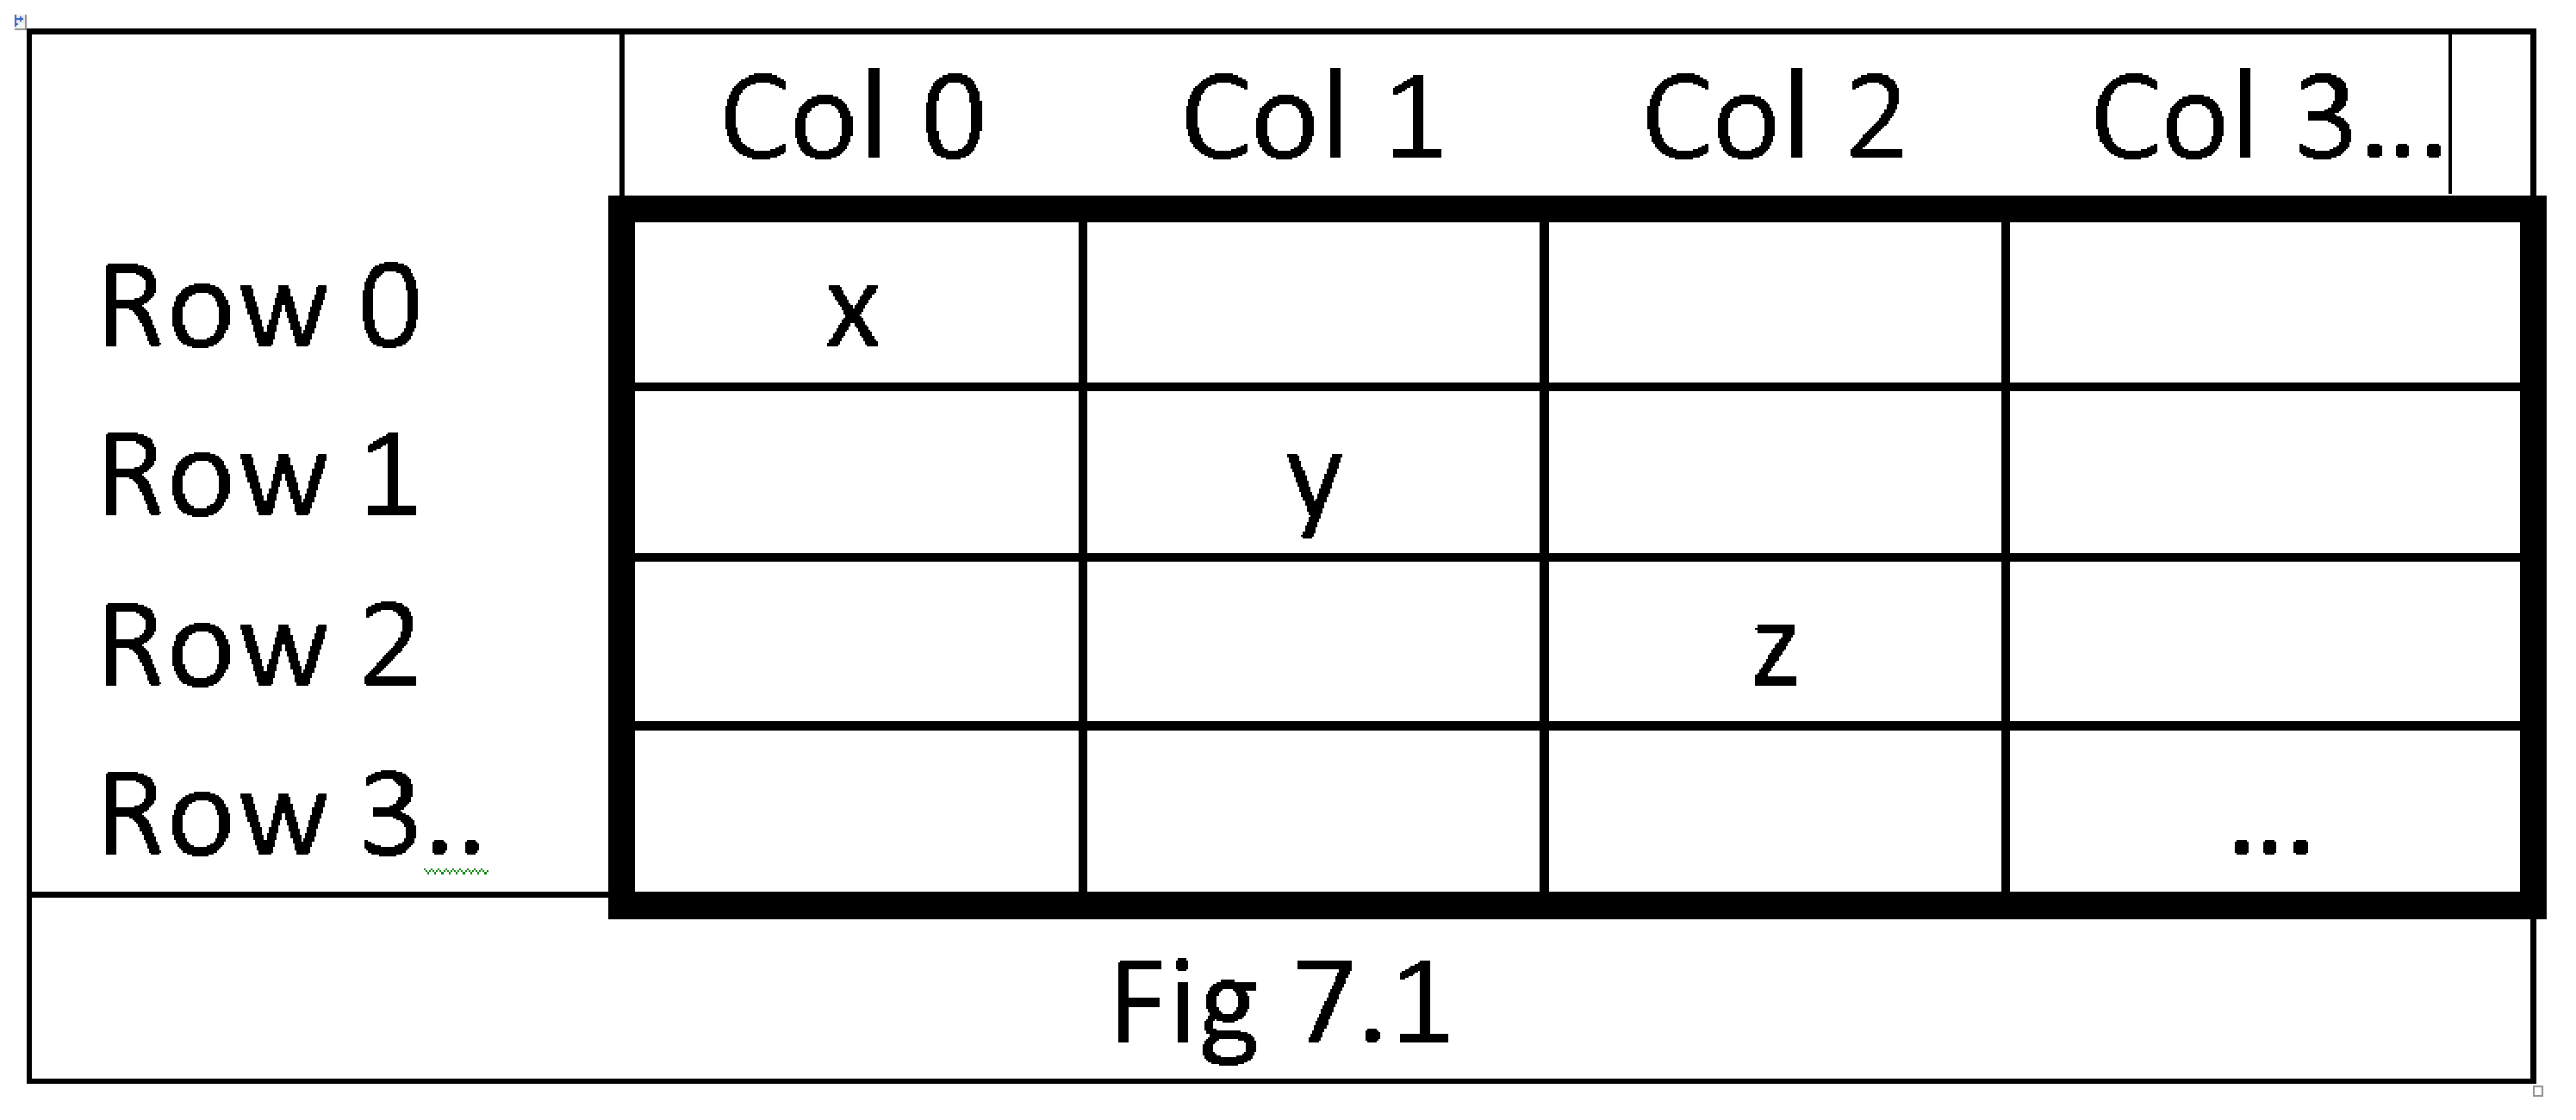
\epsfig{file=fig/Display.eps, height=1in}
\caption{The VGA display}
\label{fig:display}
\end{figure}


\subsubsection*{video.c}


The video driver is very basic and does not implement scrolling of text. For our implementation of the kprints and kprinthex we made a supplemental method call print\_char which simply sets the char for a given x, y coordinate. \\\\
What we essentially reply on is to loop though all the input text for our kprints so that it uses the print\_char with the current row we are on, while incrementing your current column so we print. As we loop through the characters of our string, we check for certain conditions. If the current row is equal to the predefined maximum row then we just set the current row to 0, so that the text simply continues from the top, or wraps around. Also if the conditions are met for either a newline character or we have reached the last column, then we increment the current row by one, and set the current column to 0.
When we need the kprinthex method we can rely on our kprints method to handle all the logic and parsing. All that is needed is to convert our hexadecimal input number into a string, and then send this string to the kprints method.
The syscall “printat” is very similar to kprints in regards to behavior, except the printat takes the initial row and column as arguments, so these are transferred via the rsi and rdi registers.
 The code is very simple and easily read - please see the project file “video.c” and “syscall.c” for further details.

\subsection{Reflections}

\subsubsection*{How would you implement support for scrolling?}
A possibility would be to have some code that would overwrite every column into the row above its immediate position.  That means that on the imaginary screen of figure~\ref{fig:display} the row 1, column 0 would be copied to row 0, column 0. This would be done with all the rows, and the ``illusion'' of scrolling would appear, and the last available row would be free to write into. Since we would be overwriting/destroying all the values in row 0, this might not be the most elegant scrolling solution, but is relatively simple and memory conserving, if not light on the CPU.\\
\\
Another solution might involve manipulation of the video pointer. A linked list could be used containing all the individual rows, with in turn contain all the columns for the individual rows. So instead of changing all the values in the rows, the linked list order is manipulated. So that if the end of the screen is reached, then the first row to display is changed from row 0 to row 1 for example. Then the last row will go from row 3 to row 0, and row 0 is cleared of values. This is a little more complicated solution, but would be more CPU load efficient compared to the previous solution. Since the video hardware reads data directly from memory, a linked list might not be technically compatible.\\
\\
The course lecture book explains another way of implementing a scrolling function, and uses a register which the video hardware is able to read, so that it has a start location for reading its input. This way we only need to increment the start location for each line as needed, and no large operations copying/moving of data are needed, since the video hardware is controlling in which order data is read, thereby lowering CPU load.
	
\label{sec:device_driver}

\section{A practical approach}
In this task we were to design and implement a real time system. The task is self-chosen.
\subsection{Traffic light}
We chose to design and implement a traffic light control system. These kind of systems are subject to real time requirements.\\
A basic model of the system can be seen in figure~\ref{fig:traffic_light}. It model as a road that has a primary road (the horisontal) and a secondary (the vertical). The primary road must be in the passable or ``green'' state as much as possible. This state is called the primary state.\\
When a car wants to cross the primary road, the light must change within a maximum amount of time. However, it sould not be possible for the secondary road to gain precedence over the primary road, if there are heavy traffic on the primary road.\\
We therefore set the following rules:
\begin{enumerate}
 \item When there are cars on the primary road, the lights cannot change to secondary state
 \item When there are no cars on the primary road, the lights can change to secondary state
 \item The light cannot be in the primary state for an unlimited amount of time
\end{enumerate}

\begin{figure}
\centering
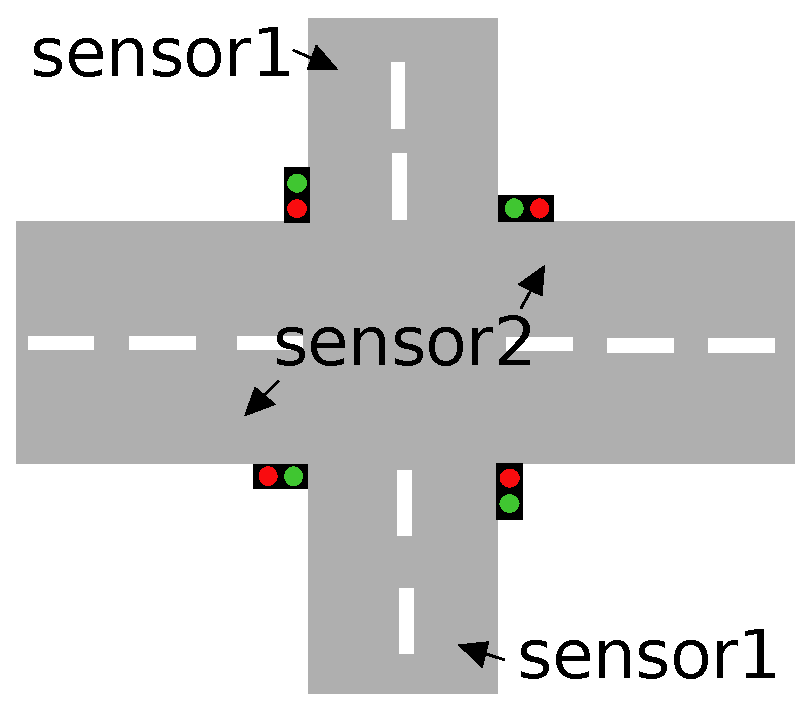
\epsfig{file=fig/Traffic_Light.eps, height=2in}
\caption{Basic model of traffic light system}
\label{fig:traffic_light}

\end{figure}

\subsection{design}
The traffic light control system has the following logic visually depicted in figure~\ref{fig:traffic_light_design}; Transition 1 only occurs if there is a no sensor input from sensor2 or the timeout has occured \emph{and} sensor1 is triggered.\\
Transition 2 occurs automatically after a timeout.

\begin{figure}
\centering
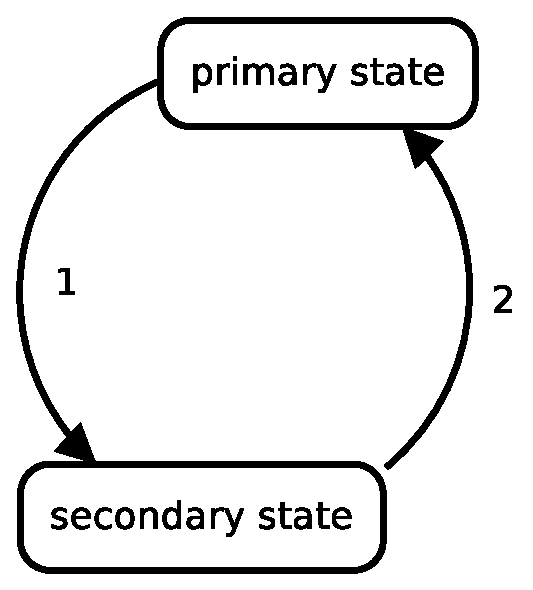
\epsfig{file=fig/Traffic_Light_Design.eps, height=2in}
\caption{States of traffic light system}
\label{fig:traffic_light_design}
\end{figure}
The real time requirements of this specification kind of resembles a sporadic scheduler, with the primary road having the highest priority, but only within a period, and then drops below the secondary roads priority. The budget is then relinquished when a change state cycle has occurred.
\subsection{Implementation}
The system consists of two processes; one process runs the sensor input part, the other does the light change. The two processes communicate via IPC (see section~\ref{sec:ipc}).\\
The light control process does most of the logic. The light state is protected with a mutex (acutally a binary semaphore), and uses three (acutally four, counting main) threads. One for recieving IPC, as this is a blocking call. One for taking care of the release policy asynchronous and one for taking care of the light switch. This thread tries to keep the mutex for itself for as long as possible. The policy thread can decide if the timer thread must give up the mutex based on the input from the IPC thread and from a ``random car generator'' used for testing.

\subsection{Test}
The test was done using visual inspection, using the graphical user interface and the debug output. The system behaved as expected, and did not change to the secondary state if cars were still arriving, but did switch if the timeout was reached or cars did not arrive.
\label{sec:practical}


\section{Conclusion}
\label{sec:conclusion}
%Conclusions; All experiences and conclusions drawn from the work.
The group widely known as group 42 would like to thank everyone for their support and free coffee.\\

\subsection{Threading}
The threading works rather well, but is very limited as it only has one thread in a process. If this was to be implemented, most of the
process handling code should be rewritten.

\subsection{Scheduling}
% ready for multithreading in processes.


%ACKNOWLEDGMENTS are optional
%\section{Acknowledgments}
%\input{acknowledgements.tex}
%Acknowledgments; Acknowledge any persons important to the work.

%References; A list of reference material used. All material must be cited in the
%text.


\appendix
\section{Work distribution}
Kim Rostgaard Christensen (s084283) 
\begin{itemize}
\item Sections: abstract, Introduction, Processes, Thread synchronization, A practical approach and Conclusion
\item Tasks: B4, A6 and B8
\end{itemize}

Andreas Rask Jensen (s083165)
\begin{itemize}
\item Sections: System calls and Interprocess communication
\item Tasks: B7 and B6
\end{itemize}

Demmus Hentze Højgaards (062591)
\begin{itemize}
\item Sections: Scheduling 4.1 and Device driver
\item Tasks: B1 and B2
\end{itemize}

Hjallgrim Gunnar Mohr Hentzes (062418)
\begin{itemize}
\item Sections: Scheduling 4.2-4 and Memory Management
\item Tasks: B3, A3 and B5
\end{itemize}




% The following two commands are all you need in the
% initial runs of your .tex file to
% produce the bibliography for the citations in your paper.
\bibliographystyle{plain}
\nocite{*}
\bibliography{sigproc}  % sigproc.bib is the name of the Bibliography in this case
% You must have a proper ".bib" file
%  and remember to run:
% latex bibtex latex latex
% to resolve all references
%
% ACM needs 'a single self-contained file'!
%
%APPENDICES are optional


%Appendixes; Appendixes holds, for example, results or figures that are not
%relevant to place in the body of the report. Appendixes should generally be
%avoided and might not be read by the course staff.


\end{document}
